\documentclass{standalone}
\usepackage{circuitikz}
\usepackage{schemabloc}

\begin{document}
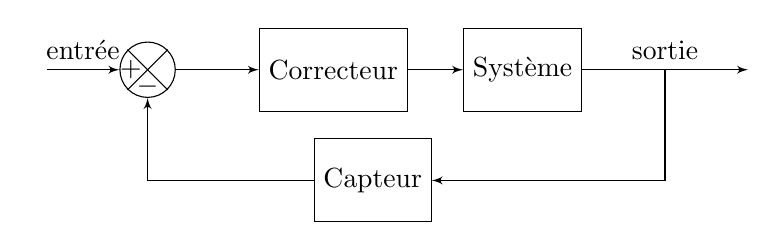
\begin{tikzpicture}
\sbEntree{E}
\sbComp{comp}{E}
\sbRelier[entrée]{E}{comp}
\sbBloc[3]{B1}{Correcteur}{comp}
\sbRelier{comp}{B1}
\sbBloc{B2}{Système}{B1}
\sbRelier{B1}{B2}
\sbSortie[6]{S}{B2}
\sbRelier[sortie]{B2}{S}
\sbDecaleNoeudy[4]{comp}{G}
\sbBloc[6]{B4}{Capteur}{G}
\sbRelieryx{B2-S}{B4}
\sbRelierxy{B4}{comp}
\end{tikzpicture}
\end{document}